\documentclass{beamer}

\usepackage{default}
\usepackage{amssymb}
\usepackage[utf8]{inputenc}

\DeclareGraphicsExtensions{{.pdf},{.png},{.jpg}}
\graphicspath{ {./img_presentation/} }

\hypersetup{colorlinks,urlcolor=blue}
\AtBeginSection[]
{
	\begin{frame}
		\begin{NoHyper}
		\tableofcontents[currentsection]
		\end{NoHyper}
	\end{frame}
}
\begin{document}
\addtobeamertemplate{footline}{\insertframenumber/\inserttotalframenumber}

	
\title{(temporal) Motifs in discussions (trees)}
\author{Alberto Lumbreras}
\date{February 17, 2016}
\maketitle

\begin{frame}\frametitle{Overview} 
\begin{NoHyper}
\tableofcontents
\end{NoHyper}
\end{frame}

\section{Introduction}
\subsection{Reddit dataset}

\begin{frame}{Reddit dataset}{A forum of forums}
	Download from:
	\href{http://couch.whatbox.ca:36975/reddit/comments/monthly/}{http://couch.whatbox.ca:36975/reddit/comments/monthly/}
	
	\vfill
	Extract forum of interest:\\
	\href{www.reddit.com/r/podemos}{www.reddit.com/r/{\color{red}science}}\\
	\href{www.reddit.com/r/podemos}{www.reddit.com/r/{\color{red}france}}\\
	\href{www.reddit.com/r/podemos}{www.reddit.com/r/{\color{red}sociology}}\\
	\href{www.reddit.com/r/podemos}{www.reddit.com/r/{\color{red}complexsystems}}\\
	\href{www.reddit.com/r/podemos}{www.reddit.com/r/{\color{red}podemos}}\\
	...
\end{frame}

\begin{frame}{Graph representations}{Graph of user interactions (a social network)}
	\begin{figure}
		\centering
		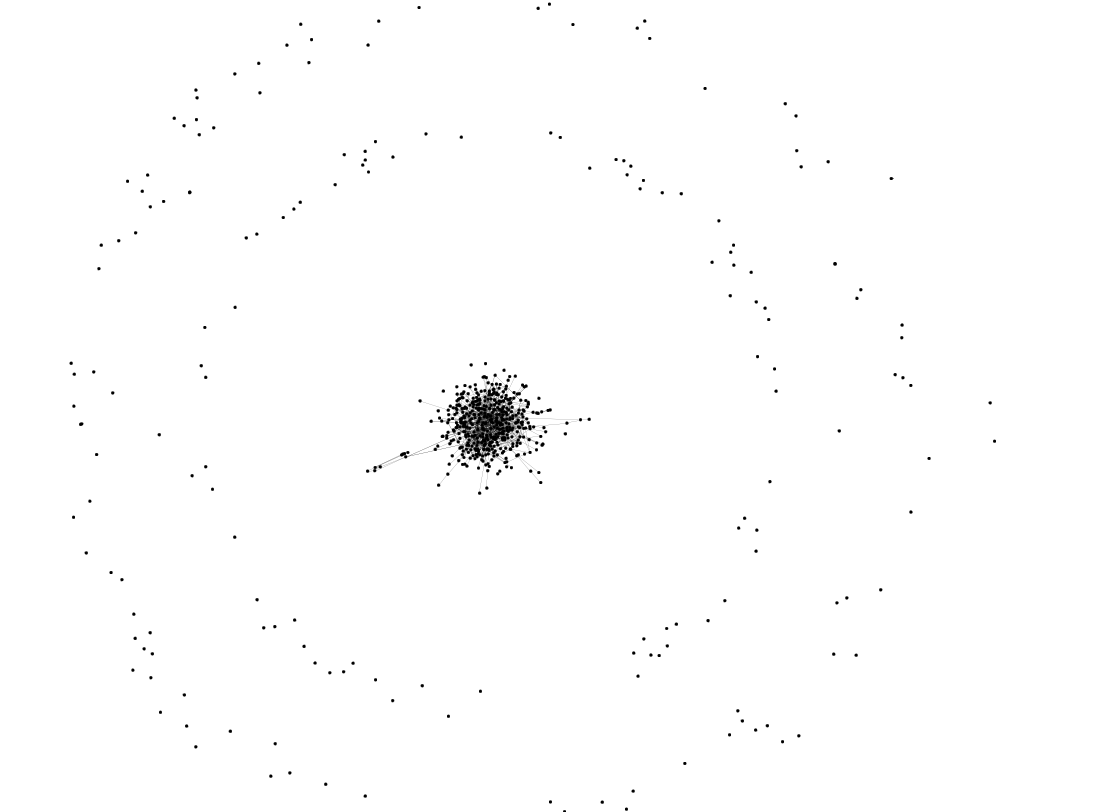
\includegraphics[width=1\textwidth]{sna}	
	\end{figure}
\end{frame}

\subsection{Graph representations}
\begin{frame}{Graph representations}{Trees of posts}
\begin{figure}
	\centering
	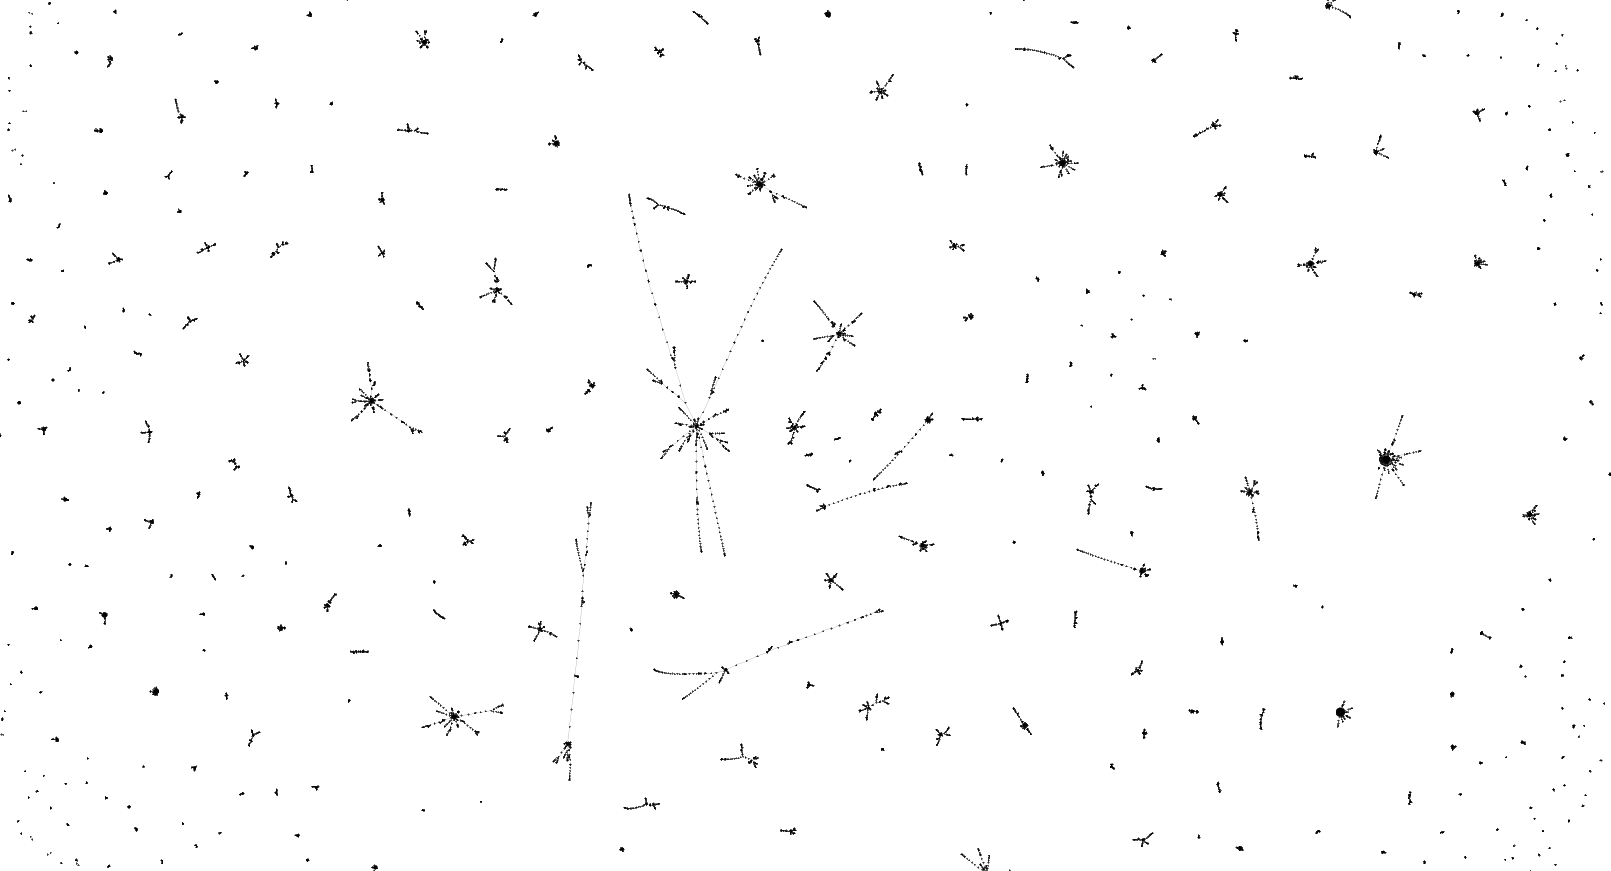
\includegraphics[width=1\textwidth]{forest}	
\end{figure}
\end{frame}

\subsection{Dynamics of conversations}
\begin{frame}{Dynamics of conversations}{Triads are not enough}
% Dibujar un arbol a la derecha
Triads in \textbf{trees of posts}:
	\begin{itemize}
		\item Only 3 possible triads (dyad, chain and star)
	\end{itemize}
	\begin{figure}
		\centering
		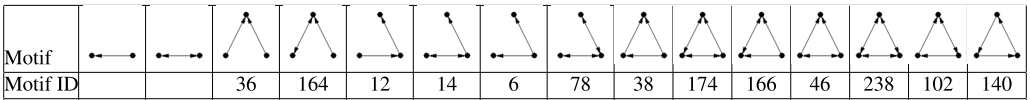
\includegraphics[width=1\textwidth]{triads}
	\end{figure}
Triads in graph of \textbf{user interactions}:
	\begin{itemize}
		\item Need of time in edges.
	\end{itemize}
\end{frame}

\begin{frame}{Temporal neighborhoods in trees}{Definition}
\begin{itemize}
	\item $N_{G}(i, d)$: neighborhood of post $i$ at distance $d$.
	\item $N_{G}(i, d, n)$: keep only the $n$ neighbors in $N_{G}(i, d)$ that are \textit{temporally} closest to post $i$ (computed as $|t-t_i|$)
	\item Keep only those posts in $N_{G}(i, d, n)$ that have a path to $i$. 
\end{itemize}

 $N_{G}(i, d, n)$ is the \textbf{temporal neighborhood} of post $i$ with distance $d$ and order $n$. \footnote{sexier names accepted}

	\begin{figure}
		\centering
		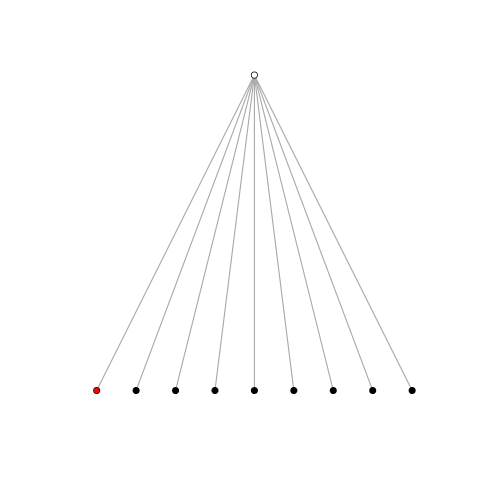
\includegraphics[width=0.5\textwidth]{large_neighborhood}
	\end{figure}
	
\end{frame}

\section{Neighborhood census}
\begin{frame}{Neighborhood census}{A real example}
Distance $d=4$ and order $n=4$. 41 discussion patterns:

\begin{figure}
	\centering
	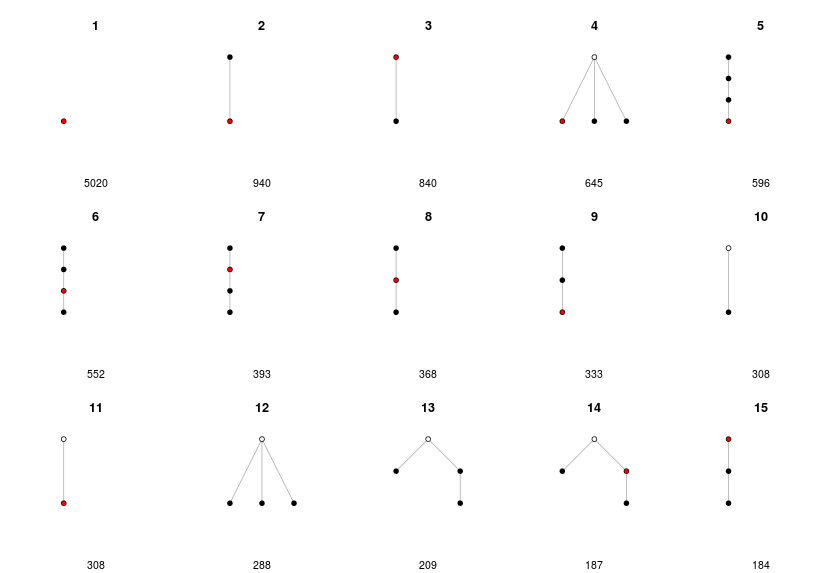
\includegraphics[width=1\textwidth]{motifs1}	
\end{figure}	
	
\end{frame}


\begin{frame}{Neighborhood census}{Cyclic dynamics}

\begin{figure}
	\centering
	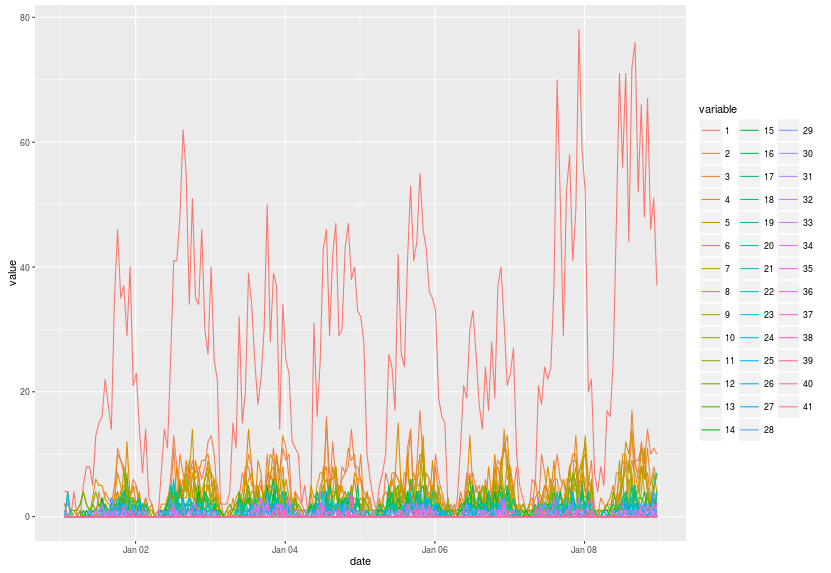
\includegraphics[width=1\textwidth]{motifs_by_hour}	
\end{figure}
\end{frame}


\begin{frame}{Neighborhood census}{Proportions}
	\begin{figure}
		\centering
		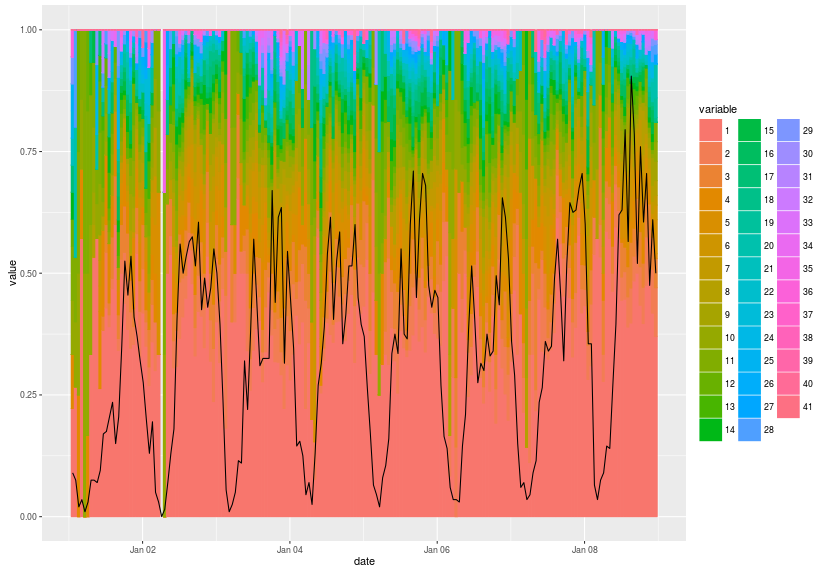
\includegraphics[width=1\textwidth]{census_proportions}	
	\end{figure}
\end{frame}

\begin{frame}{Neighborhood census}{Census and thread growth}
	\begin{figure}
		\centering
		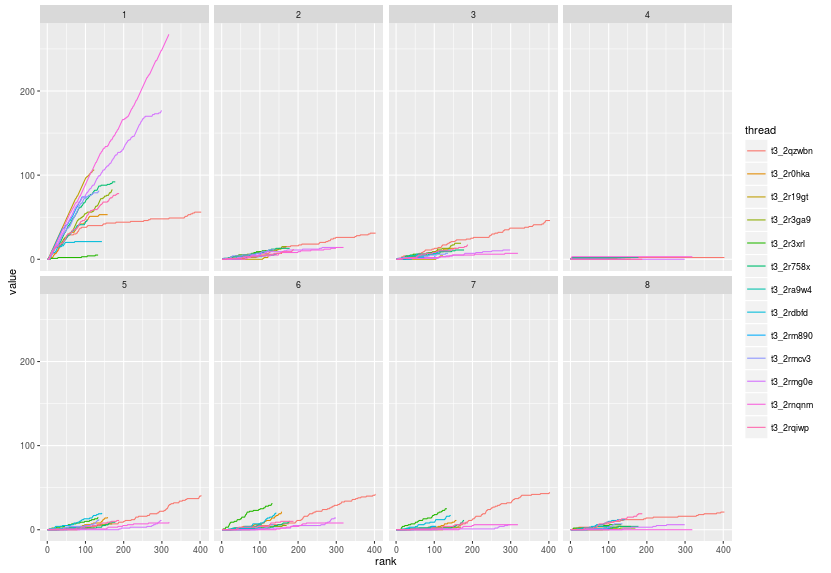
\includegraphics[width=1\textwidth]{census_length}	
	\end{figure}
\end{frame}

\begin{frame}{Neighborhood census}{Predictions}
	\textbf{Q}: Can we predict whether a thread will succeed based on its initial structure (neighborhoods)?\\
	\textbf{A}: ...\textit{the answer in a few hours}
\end{frame}
\section{You are the way you (structurally) talk?}
\begin{frame}{Neighborhood-based clustering}{Overview}
\begin{itemize}
	\item Create a user $\times$ neighborhood matrix of counts.
	\item Z-normalize (users characterized by their deviation from the mean)
	\item Cluster!
\end{itemize}
\end{frame}


\begin{frame}{Neighborhood-based clustering}{Uncolored neighborhoods}
	\begin{figure}
		\centering
		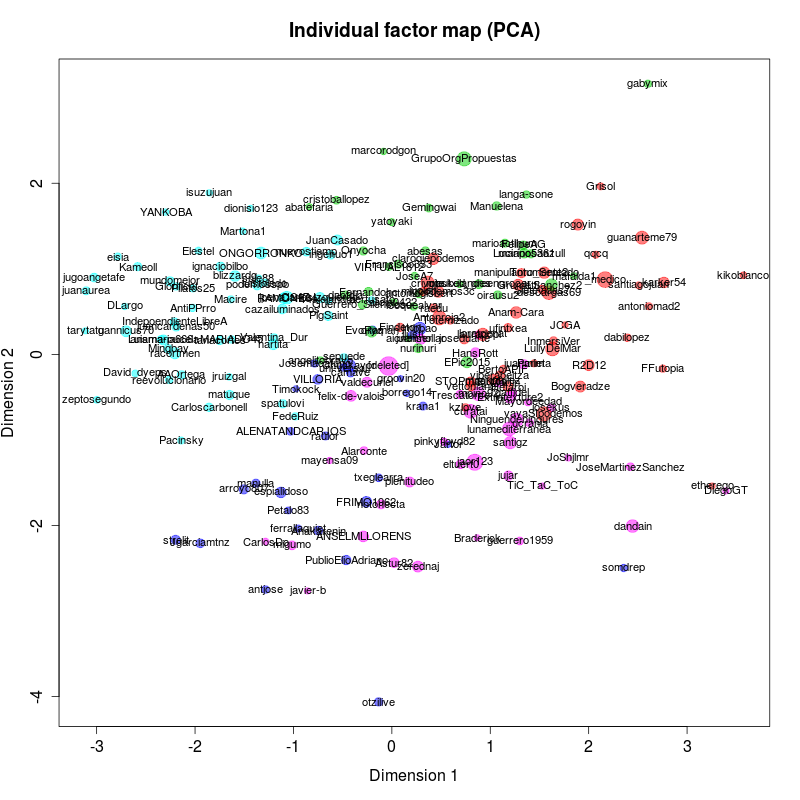
\includegraphics[width=0.75\textwidth]{PCA_nocolor}
	\end{figure}	
\end{frame}

\begin{frame}{Neighborhood-based clustering}{Uncolored neighborhoods}
	$k$-means suggests 5 groups:
	\begin{figure}
		\centering
		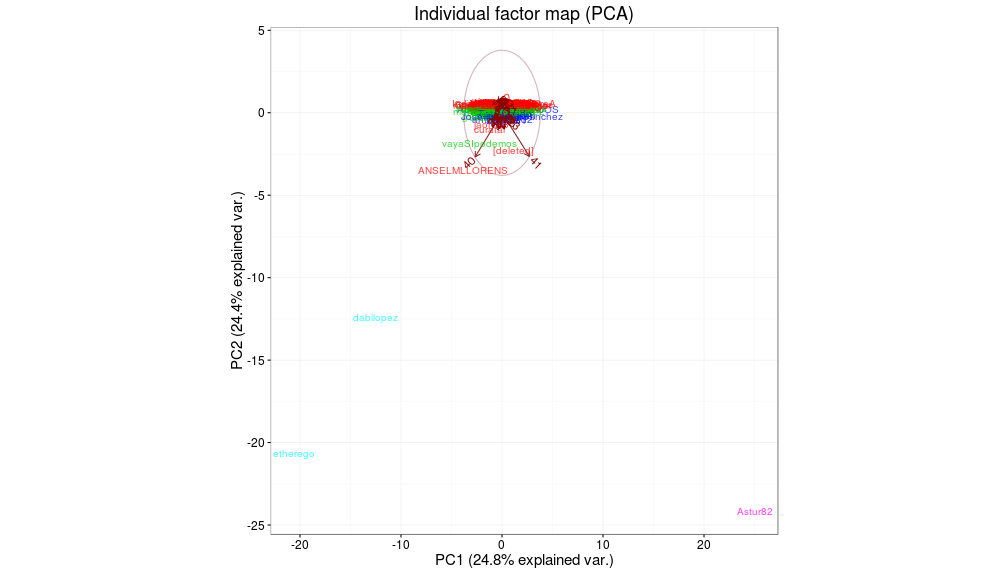
\includegraphics[width=1\textwidth]{PCA}%
	\end{figure}	
\end{frame}


\begin{frame}{Neighborhood-based clustering }
	\begin{figure}
		\centering
		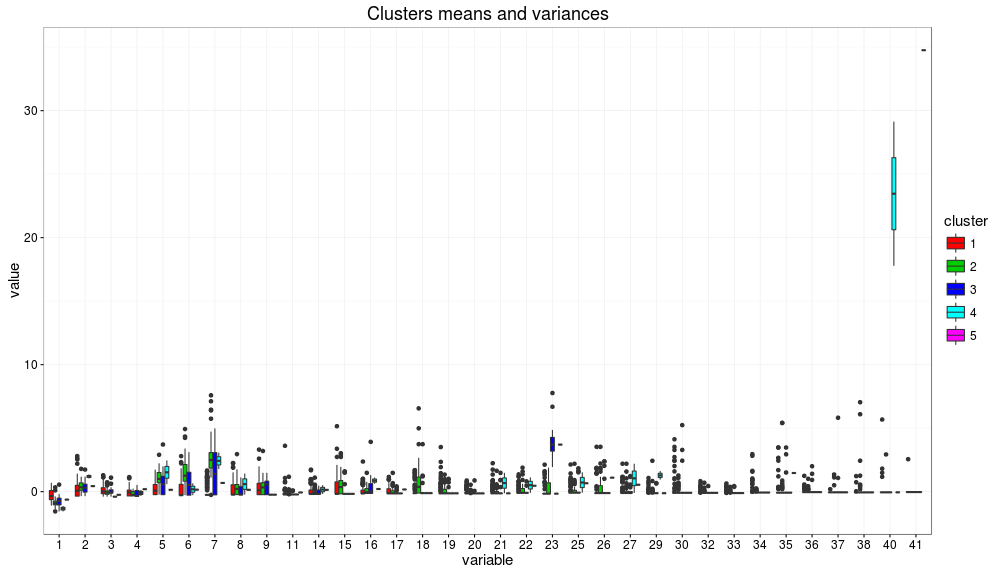
\includegraphics[width=1\textwidth]{whiskers}	
	\end{figure}
\end{frame}



\section{Conclusions}
\begin{frame}{Conclusions}
	\begin{itemize}
			\item Temporal neighborhoods richer than triads to analyze the structure of conversations.
			\item Users can be characterized in terms of what type of neighborhood they participate in (or they trigger).
	\end{itemize}
	Future work:
	\begin{itemize}
		\item Do users jump from cluster to cluster (paths of roles)
		\item Are initial census predictive of the success of a discussion?.
	\end{itemize}	

\end{frame}
\end{document}